\documentclass{article}
\iffalse
This file is protected by Copyright. Please refer to the COPYRIGHT file
distributed with this source distribution.

This file is part of OpenCPI <http://www.opencpi.org>

OpenCPI is free software: you can redistribute it and/or modify it under the
terms of the GNU Lesser General Public License as published by the Free Software
Foundation, either version 3 of the License, or (at your option) any later
version.

OpenCPI is distributed in the hope that it will be useful, but WITHOUT ANY
WARRANTY; without even the implied warranty of MERCHANTABILITY or FITNESS FOR A
PARTICULAR PURPOSE. See the GNU Lesser General Public License for more details.

You should have received a copy of the GNU Lesser General Public License along
with this program. If not, see <http://www.gnu.org/licenses/>.
\fi

\author{} % Force author to be blank
%----------------------------------------------------------------------------------------
% Paper size, orientation and margins
%----------------------------------------------------------------------------------------
\usepackage{geometry}
\geometry{
	letterpaper,			% paper type
	portrait,				% text direction
	left=.75in,				% left margin
	top=.75in,				% top margin
	right=.75in,			% right margin
	bottom=.75in			% bottom margin
 }
%----------------------------------------------------------------------------------------
% Header/Footer
%----------------------------------------------------------------------------------------
\usepackage{fancyhdr} \pagestyle{fancy} % required for fancy headers
\renewcommand{\headrulewidth}{0.5pt}
\renewcommand{\footrulewidth}{0.5pt}
\rhead{\small{ANGRYVIPER Team}}
%----------------------------------------------------------------------------------------
% Appendix packages
%----------------------------------------------------------------------------------------
\usepackage[toc,page]{appendix}
%----------------------------------------------------------------------------------------
% Defined Commands & Renamed Commands
%----------------------------------------------------------------------------------------
\renewcommand{\contentsname}{Table of Contents}
\renewcommand{\listfigurename}{List of Figures}
\renewcommand{\listtablename}{List of Tables}
\newcommand{\todo}[1]{\textcolor{red}{TODO: #1}\PackageWarning{TODO:}{#1}} % To do notes
\newcommand{\code}[1]{\texttt{#1}} % For inline code snippet or command line
%----------------------------------------------------------------------------------------
% Various pacakges
%----------------------------------------------------------------------------------------
\usepackage{hyperref} % for linking urls and lists
\usepackage{graphicx} % for including pictures by file
\usepackage{listings} % for coding language styles
\usepackage{rotating} % for sideways table
\usepackage{pifont}   % for sideways table
\usepackage{pdflscape} % for landscape view
%----------------------------------------------------------------------------------------
% Table packages
%----------------------------------------------------------------------------------------
\usepackage{tabularx} % c=center,l=left,r=right,X=fill
\usepackage{float}
\floatstyle{plaintop}
\usepackage[tableposition=top]{caption}
\newcolumntype{P}[1]{>{\centering\arraybackslash}p{#1}}
\newcolumntype{M}[1]{>{\centering\arraybackslash}m{#1}}
%----------------------------------------------------------------------------------------
% Block Diagram / FSM Drawings
%----------------------------------------------------------------------------------------
\usepackage{tikz}
\usetikzlibrary{shapes,arrows,fit,positioning}
\usetikzlibrary{automata} % used for the fsm
%----------------------------------------------------------------------------------------
% Colors Used
%----------------------------------------------------------------------------------------
\usepackage{colortbl}
\definecolor{blue}{rgb}{.7,.8,.9}
\definecolor{ceruleanblue}{rgb}{0.16, 0.32, 0.75}
\definecolor{drkgreen}{rgb}{0,0.6,0}
\definecolor{deepmagenta}{rgb}{0.8, 0.0, 0.8}
\definecolor{cyan}{rgb}{0.0,0.6,0.6}
\definecolor{maroon}{rgb}{0.5,0,0}
%----------------------------------------------------------------------------------------
% Update the docTitle and docVersion per document
%----------------------------------------------------------------------------------------
\def\docTitle{Component Data Sheet}
\def\docVersion{1.3}
%----------------------------------------------------------------------------------------
\date{Version \docVersion} % Force date to be blank and override date with version
\title{\docTitle}
\lhead{\small{\docTitle}}

\def\comp{matchstiq\_z1\_i2c}
\edef\ecomp{matchstiq_z1_i2c}
\def\Comp{Matchstiq-Z1 I2C}
\graphicspath{ {figures/} }

\begin{document}

\section*{Summary - \Comp}
\begin{tabular}{|c|M{13.5cm}|}
	\hline
	\rowcolor{blue}
	                  &                                        \\
	\hline
	Name              & \comp                                  \\
	\hline
	Worker Type       & Device                                 \\
	\hline
	Version           & v\docVersion \\
	\hline
	Release Date      & February 2018 \\
	\hline
	Component Library & ocpi.assets.platforms.matchstiq\_z1.devices \\
	\hline
	Workers           & \comp.hdl                              \\
	\hline
	Tested Platforms  & Matchstiq-Z1(PL)                       \\
	\hline
\end{tabular}

\section*{Worker Implementation Details}
The Matchstiq-Z1 I2C device worker uses the subdevice construct to implement the I2C bus for the Matchstiq-Z1 platform. Matchstiq-Z1 I2C supports 5 device workers:
\begin{enumerate}
	\item Si5338
	\item Matchstiq-Z1 AVR
	\item Pca9534
	\item Pca9535
	\item Tmp100
\end{enumerate}
Matchstiq-Z1 I2C uses the i2c primitive library which is based upon the OpenCores I2C controller. This revision of the device worker supports 8 bit and 16 bit I2C accesses.

\section*{Block Diagrams}
\subsection*{Top level}
\begin{figure}[ht]
	\centerline{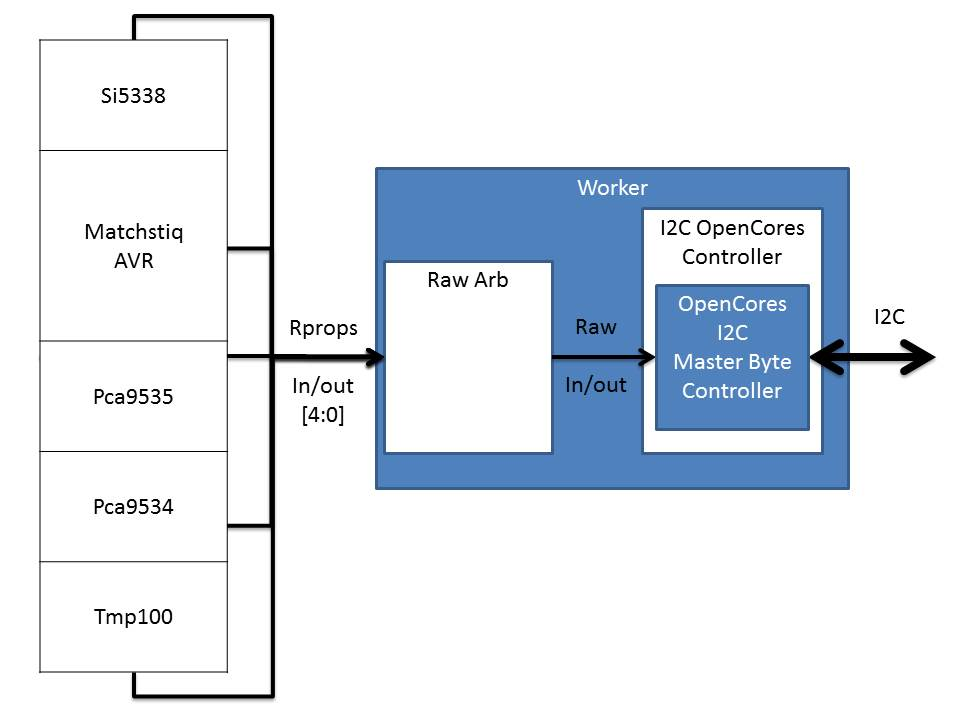
\includegraphics[scale=0.4]{block_diagram}}
	\caption{I2C Connection Block Diagram}
	\label{fig:tb}
\end{figure}
\subsection*{State Machine}
\begin{figure}[ht]
	\centerline{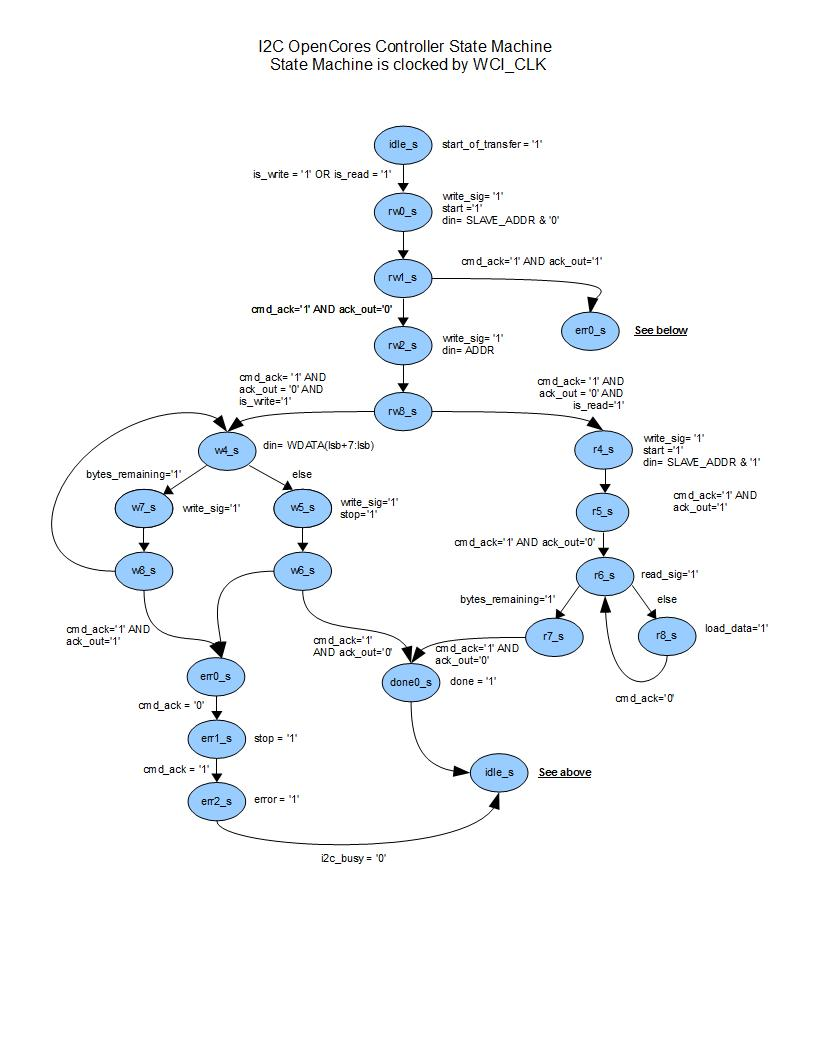
\includegraphics[scale=0.6]{state_machine_diagram}}
	\caption{I2C OpenCores Controller State Machince}
	\label{fig:tb}
\end{figure}

\section*{Source Dependencies}
\subsection*{\comp.hdl}
\begin{itemize}
	\item ocpi.assets/hdl/platforms/matchstiq\_z1/\comp.hdl/\comp.vhd
	\item ocpi.assets/hdl/primitives/i2c/i2c\_pkg.vhd
	      \begin{itemize}
	      	\item ocpi.assets/hdl/primitives/i2c/i2c\_opencores\_ctrl.vhd
	      	\item ocpi.assets/hdl/primitives/i2c/i2c\_master\_byte\_ctrl.v
	      	\item ocpi.assets/hdl/primitives/i2c/i2c\_master\_bit\_ctrl.v
	      	\item ocpi.assets/hdl/primitives/i2c/timescale.v
	      	\item ocpi.assets/hdl/primitives/i2c/i2c\_master\_defines.v
	      \end{itemize}
	\item ocpi.core/hdl/primitives/ocpi/raw\_arb.vhd
\end{itemize}

\begin{landscape}
\section*{Component Spec Properties}
	\begin{scriptsize}
		\begin{tabular}{|p{3cm}|p{1.5cm}|c|c|c|c|c|p{7cm}|}
			\hline
			\rowcolor{blue}
			Name                   & Type   & SequenceLength & ArrayDimensions & Accessibility       & Valid Range & Default & Usage                        \\
			\hline
			\verb+NUSERS_p+        & -      & -              & -               & Readable, Parameter & -           & 5       & Number of supported devices     \\
			\hline
			\verb+SLAVE_ADDRESS_p+ & UChar  & -              & \verb+NUSERS_p+ & Readable, Parameter & -           & -       & Array of I2C Slave Addresses \\
			\hline
			\verb+CLK_FREQ_p+       & Float & -              & -               & Readable, Parameter & -           & 100e6 & Input clock rate which is divided down to create I2C clock  \\
			\hline
		\end{tabular}
	\end{scriptsize}

	\section*{Worker Interfaces}
	\subsection*{\comp.hdl}
	\begin{scriptsize}
		\begin{tabular}{|M{2cm}|M{1.5cm}|c|c|M{6cm}|}
			\hline
			\rowcolor{blue}
			Type & Name & DataWidth & Advanced & Usage \\
			\hline
			RawProp
			& rprops
			& -
			& Count=\verb+NUSERS_p+ Optional=true
			& \begin{flushleft}Raw properties connections for master devices \newline Index 0: matchstiq\_z1\_avr \newline Index 1: si5338 \newline Index 2: tmp100 \newline Index 3: pca9534 \newline Index 4: pca9535 \end{flushleft}\\
			\hline
		\end{tabular}
	\end{scriptsize}

	\section*{Signals}
	\begin{scriptsize}
	\begin{tabular}{|c|c|c|c|p{2.6cm}|c|c|c|}
		\hline
		\rowcolor{blue}
		Name & Type  & Width & Description \\
		\hline
		SDA  & Inout & 1     & I2C Data    \\
		\hline
		SCL  & Inout & 1     & I2C Clock   \\
		\hline
	\end{tabular}
	\end{scriptsize}
\end{landscape}

\section*{Control Timing and Signals}
The Matchstiq-Z1 I2C HDL device worker uses the clock from the Control Plane and standard Control Plane signals.

\section*{Performance and Resource Utilization}
\subsubsection*{\comp.hdl}
\input{../../\ecomp.hdl/utilization.inc}
\section*{Test and Verification}
Testing of the Matchstiq-Z1 I2C device worker consists of a C++ test bench that use the Application Control Interface API to command the UUT.
% simulation section belongs in a differnt doc, leaving commented out so we dont lose content
% As the simulation (i2c_sim.test/) is generic, it was moved to hdl/devices/.
%\subsubsection*{Simulation}
%The simulation test bench is based on a simulation model of an I2C slave.
%Workers analagous to the Matchstiq-Z1 I2C component and the workers it supports were developed based on the simulation model.
%The slave has 4 8-bit registers and a user configurable slave address. The testbench performs a write and readback test for each type of worker it supports. The following shows the console output of a successful run of the testbench.\par\bigskip
%\noindent \texttt{App initialized.\\
%App started.\\
%App stopped.\\
%I2C Readback Test for 8 bit master: Passed.\\
%I2C Readback Test for 16 bit master: Passed.\\
%I2C Readback Test for 8 bit mixed master: Passed.\\
%I2C Readback Test for 16 bit mixed master: Passed.\\
%I2C Readback Test for 16 bit extended write master: Passed.\\
%I2C Sim Testbench: Passed.}\par\bigskip
%\noindent Should all tests pass a file i2c\_sim\_testbench.results is produced for use with automated testing.
\subsubsection*{Hardware}
\begin{flushleft}
Hardware testing of the Matchstiq-Z1 I2C device worker consists of connecting the Matchstiq-Z1 RX SMA panel to a signal generator before running the testbench.
The signal generator should be set to 2.140001 GHz at -55 dBm.\\
Building the testbench assumes that the Matchstiq-Z1 platform has been built. Details on how to build the Matchstiq-Z1 platform can be found in the Matchstiq-Z1 platform document.\\
The testbench checks the functionality of the I2C devices and generates an output file (odata/testbench\_rx.out) with the received input data. Should the testbench complete successfully (AVR serial number = 6026), a file i2c\_hw\_testbench.results is produced for use with automated testing. Figure 1 shows the expected result for the received data. These results should be inspected manually as the testbench does not verify these trends.\par\bigskip
	\begin{figure}[ht]
		\centerline{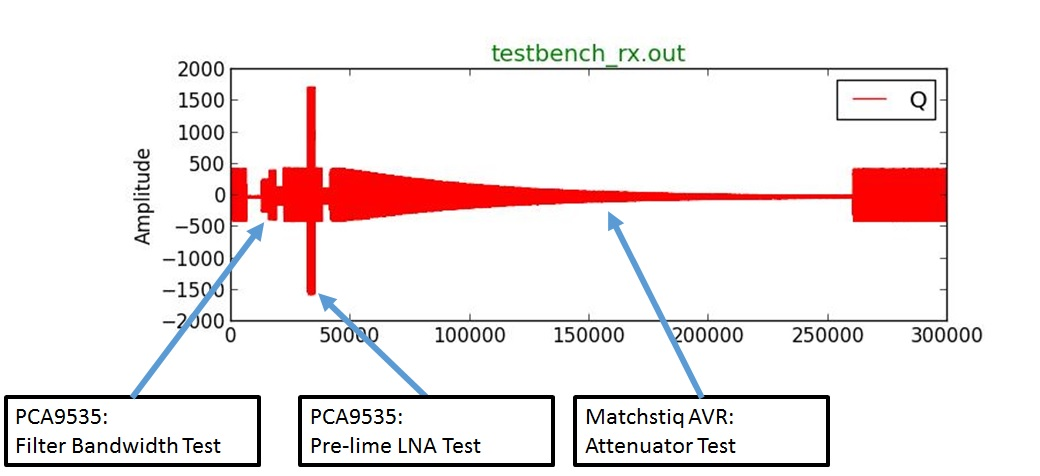
\includegraphics[scale=0.5]{testbench_rx}}
		\caption{Expected Results}
		\label{fig:tb}
	\end{figure}
\end{flushleft}

\section*{References}
\begin{flushleft}
	\begin{itemize}
		\item[1)] The Matchstiq-Z1 Software Development Manual (provided by Epiq with the Platform Development Kit)
	\end{itemize}
\end{flushleft}
\end{document}
